\chapter{Conclusiones y vías futuras}

Llegados a este punto se puede decir que los objetivos han sido realizados. La rigidez de ovaloides a sido demostrada y la visualización de superficies a sido programada.
${ }$\\

Mientras realizaba este trabajo me han ido surgiendo algunas dudas acerca de la rigidez y los ovaloides, algunas de ellas son: 
${ }$\\

\begin{itemize}
	\item A parte de los ovaloides, ¿hay mas superficies que sean rígidas? ¿Podríamos imaginar una superficie en la que en algunos de sus puntos la curvatura sea negativa pero esta superficie sea rígida?
	
	\item Superficies compactas y conexas con curvatura positiva en todos sus puntos no pueden ser deformadas por isometrías, analizando visualmente ese hecho sobre superficies mas simples como son las esferas se puede intuir por que la forma que toman estas superficies con curvatura positiva no pueden ser deformadas por funciones que mantienen la longitud de las curvas. ¿Sería posible a partir de esta intuición encontrar otras superficies rígidas que no sean ovaloides? La Figura \ref{fig:etiq_21} muestra un toro, a simple vista pudiera parecer rígido, ¿es realmente rígido?.
	
	\item En contraste con el apartado anterior la superficie vista anteriormente en la Figura \ref{fig:etiq_2} tiene curvatura negativa en algunos de sus puntos pero no es rígida. Esto se debe, como hemos dicho antes, a que existe un plano a través del cual podemos hacer el simétrico de los puntos que se encuentran en uno de los semi-espacios definidos por él. ¿Pudiera ser, que las únicas figuras conexas y compactas que no son rígidas, son aquellas para las que existe un plano con las mismas características que se mencionan en la figura anterior?
	
	\item ¿Se ha estudiado ya acerca de como generalizar el teorema de rigidez de ovaloides? Mientras intentaba encontrar información acerca de la rigidez de superficies me he encontrado con bibliografía que parece generalizar el resultado de Cohn-Vossen. Por ejemplo, en la página web \cite{ref7} encontré el libro \cite{math1} que me gustaría mirar mas en profundidad. También encontré un libro con un capítulo que hablaba acerca de tres tipos de rigidez del cual no recuerdo el título.
	
	\item ¿Tiene la rigidez de superficies una aplicación en la vida real?¿O en alguna otra ciencia como la física?
\end{itemize}
${ }$\\

	\begin{figure}[h]
		\begin{center}
			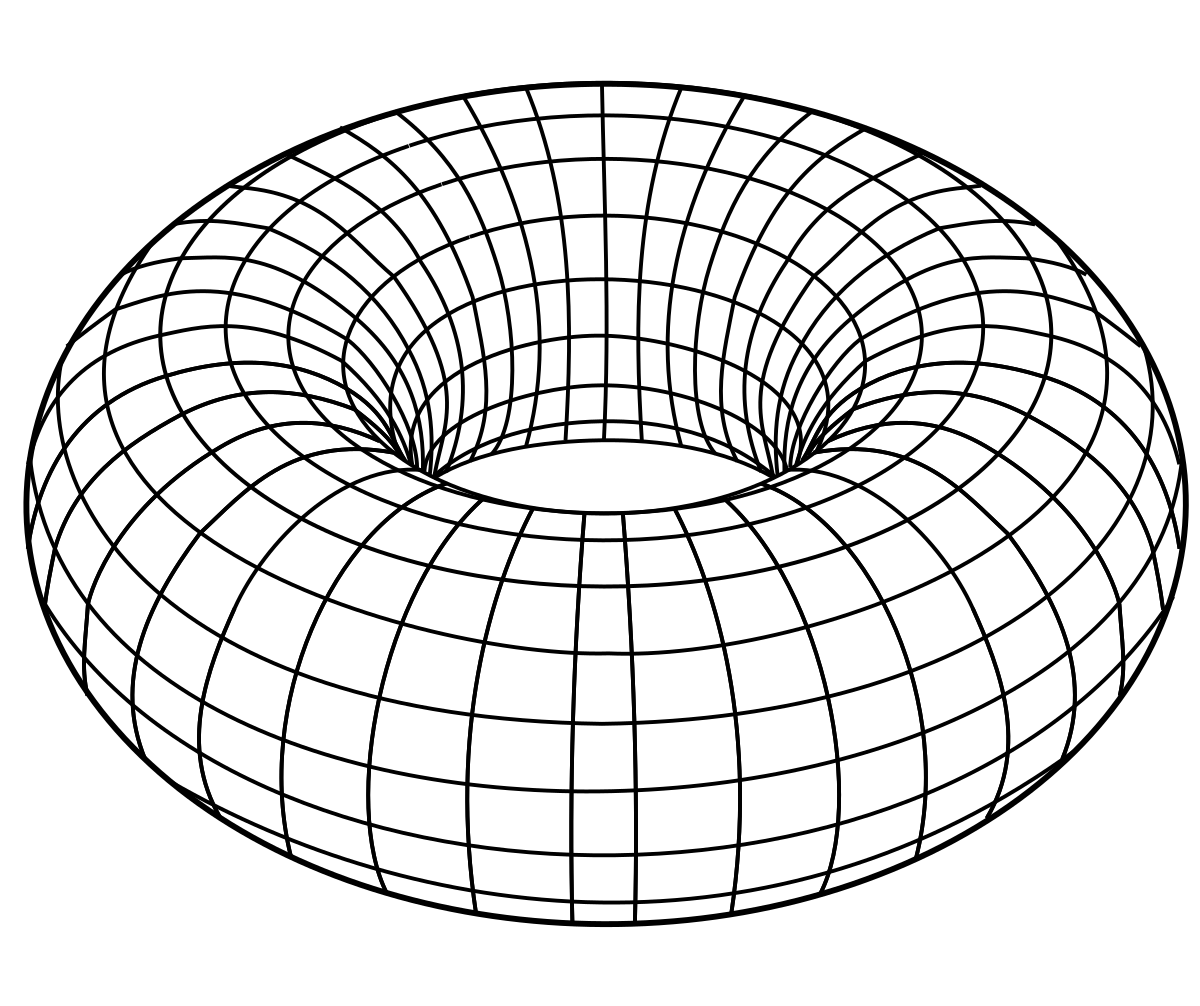
\includegraphics[width=0.6\textwidth]{imagenes/toro.png}
		\end{center}
		\caption{Toro superficie con curvatura negativa en algunos de sus puntos pero rígido.}
		\label{fig:etiq_21}
	\end{figure}


Con respecto a la parte de visualización, me hubiese gustado haber implementado las texturas para que las imágenes fuesen mejores y haber hecho que funcionase para mas de una fuente de luz. Por otro lado, también me gustaría que fuese posible mover la cámara y que fuese mas interactivo. Por ejemplo, dar al usuario la posibilidad de elegir el tipo de figura a mostrar y de ajustar las constantes de las ecuaciones implícitas.
${ }$\\

Buscando en internet encontré una forma de modelar las superficies que usa la función distancia de objetos sencillos y sobre estos se realizan modificaciones para crear superficies mas complejas. Esto se puede ver los artículos de Inigo Quilez que podemos encontrar en el enlace \cite{IQuilez}.


